\documentclass[final]{rapport1}
\usepackage[utf8]{inputenc}
\usepackage[export]{adjustbox} 
\usepackage{pdfpages}
\usepackage{graphicx}
\usepackage{authblk}
\usepackage[danish]{babel}
\usepackage{csquotes}
\usepackage[nottoc]{tocbibind}
\addto{\captionsdanish}{\renewcommand{\abstractname}{Abstract}}


\begin{document}
\begin{titlepage}
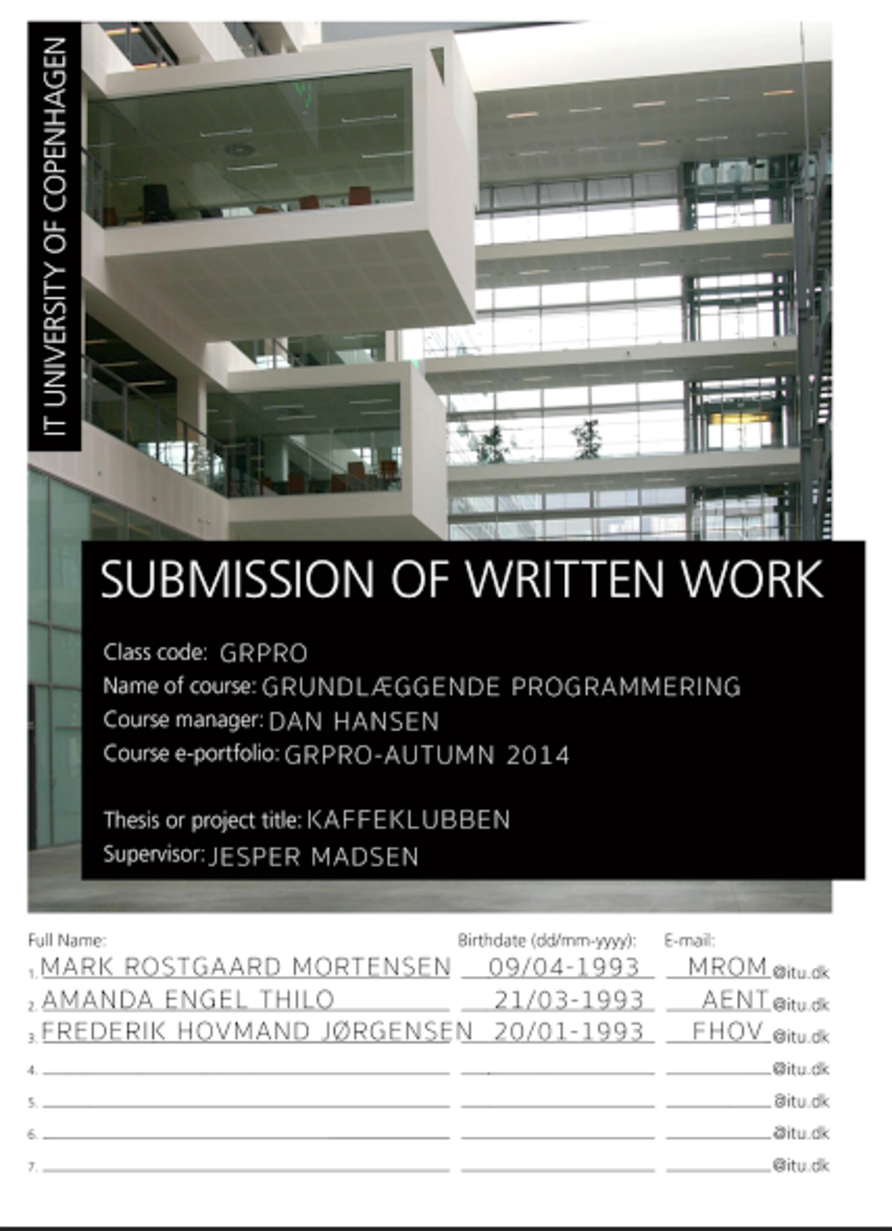
\includepdf{frontpage.pdf}
\end{titlepage}



\includepdf[width=400pt]{forside.pdf}



 
\baselineskip= 15pt

\begin{abstract}

In this report we address our workgroups attempt at designing a digital solution for broadening the audience for both the digital and physical offerings, that Statens Museum for Kunst(SMK) provides. We use a multitude of idea generation techniques, to arrive at a product, and then interviews with SMK. We propose an enhanced web-presence, for image viewing and discussion, based on feedback from SMK and visits to the museum. The report concludes with the proposal of a system in which users can comment and interact with the different artworks on the website.

\end{abstract}
\clearpage
\tableofcontents
\chapter{Forord}


\chapter{Indledning}
\section{Baggrund}
Det problemområde vi har arbejdet med i forbindelse med vores projekt, er udviklingen af et softwaresystem til brug for en ekspedient der betjener en billetluge i en biograf. Det område der skulle dækkes var reservation både når kunden stod foran billetlugen, samt når kunden ringede ind på telefon. Vores løsning skulle håndtere   ekspedientens arbejdsopgaver i sådanne situationer. Løsningen skal derfor fokusere udelukkende på reservationer, og ikke salg. 

\section{Problemstilling}

\subsection{Krav til programmet}
Af krav til porgrammet kan nævnes at der i forbindelse med reservationerne skal oplyses navn eller anden identitet på kunden. Vi har i vores program valgt at den centrale inforamtion omkring brugeren er dennes telefonnummer. Det har vi gjort af den grund af flere kunder godt kan have samme navn, men at ens telefonnummer er unikt.  

Derudover skal biografen indeholde flere sale, og sende flere forskellige forestillinger i løber af dagen. Salenes størrese, antal pladser mm, skal fremgå af databsen frem for at være indkodet i selve programteksten. Derfor har vi istædet for at skrive data ind i programteksten, valgt at lave en speciel klasse til at hente data fra databasen. 

Det samme er gældende for de enkelte forestillinger, der derfor også bliver gemt i databasen.

\subsection{Brugerscenario}
Når ekspedienten åbner vores biobooking-system vil der på venstre side af vinduet vare oplistet de film der spilledes i biografen i øjeblikket. Klikker ekspedienten på en af disse film vil der på højre side af vinduet vise sig de tilhørende spilletider til den valgte film. Klikker ekspedienten derimod ikke på noget, vil der til stå følgene tekst \emph{Klik på en film til venstre for at vise tidspunkter}. Øverst oppe i vinduet vil man se tre faner: \emph{Forestillinger, Reservation og Ret reservation}. Man kan godt navigere mellem fanerne, men har man ikke først valgt film og tidspunkt vil \emph{Reservation} være ubrugelige.
 
Efter at ekspedienten har valgt en film og en spilletid vil systemet automatisk skifte videre til den næste fane: \emph{Reservation}. Her kan ekspedienten vælge fri mellem de ledige sæder. Dette gøres ved at ekspedienten enten klikker enkeltvis på de grønne sæder, eller ved at trække musen over de ønskede sæder. De valgte sæder vil nu blive blå, så ekspedienten kan se hvilke der er valgt. Er sæderne tilfredsstillende skal ekspedienten skive navn samt telefonnummer på kunden ind i et informationsfelt nedernst til højre på siden. Nederst på siden ses i venstre hjørne antallet af sæder i alt, samt det ledige antal sæder. Dette kan ekspedienten også se på det grafiske billede over biografsalen, da de allerede reserverede sæder er røde, samt umulige at vælge for reservation. Efter kundens information er indtastet og ekspedienten har klikket på \emph{Fuldfør reservation} knappen kommer et pop-up vindue op, hvor der står skrevet: \emph{Bestillingen er gennemførst}.

Ønsker den pågældende kunde derimod at ændre eller slette en reservation, skal ekspedienten klikke sig ind på den sidste fane: \emph{Ret reservation}. På denne side finder ekspedienten øverst opppe et indput felt hvor kundens telefonnumer skal indtastes. Når ekspedienten har klikket enter vil kundens reservation(er) dukke op nedenfor i en pæn liste. Ekspedienten kan så klikke på den reservation som kunden ønsker ændret. Nu føres ekspedienten tilbage til \emph{Reservation} fanen, men de sæder tilknyttet den pågældende reservation ses nu med blåt frem for rødt. Ekspedienten kan således tilføje eller fjerne sæder ved at klikke på sæder med musem og derefter klikke på \emph{Ret reservation} knappen. Ønsker kunden helt at slette reservationen kan dette lade sig gøre ved at klikke på \emph{Slet reservation} knappen. 

\subsection{Systemdesign}



\chapter{Problemanalyse}
\section{Vores løsning}

\subsection{Alternative løsninger}

\section{Databasedesign}


%\begin{picture}

%\includegraphics[width=300pt]{minverva.png}

%\end{picture}
%\begin{center}
%\tiny Figure 1. Minerva modellen
%\linebreak
%\linebreak
%\linebreak
%\end{center}


\chapter{Brugervejledning}
\section{Programmet - hvordan fungere det}

\subsection{Begrænsninger}
\subsection{Fejlmeddelsesr}
\section{Eksempel}

\clearpage
\chapter{Problemanalyse}

\chapter{Løsning}
\section{Teknisk Analyse}
\subsection{Kommentarsystem}


\subsection{Crowd-sourcet}

\subsection{Single Page Application}

\subsection{Backend}

\subsection{Programmeringssprog}
\begin{itemize}
\item 
\item 
\item 
\item 
\item 
\end{itemize}

\subsection{White- og Blackbox testing}

\subsection{Application Programming Interface(API)}
\clearpage
\section{Design}

\subsection{Index side}

\subsection{Værkforum}



\subsection{Zoomfuktion}


\section{Teknisk beskrivelse}
\subsection{Flowchart}

\subsection{Data}
\begin{itemize}
\item 
\item
\item 
\begin{itemize}
\item 
\item 
\end{itemize}
\end{itemize}

\subsection{Arkitektur}
\begin{itemize}
\item 
\item 
\end{itemize}

\subsection{Brugergrænseflade}
\subsubsection{Lyttere}

\subsubsection{Komponenter}


\subsection{Begrænsninger}

\chapter{Afprøvning}

\begin{enumerate}
\item 
\item 
\item 
\item

\end{enumerate}

\chapter{Brugervejledning}
\section{Eksempel}

\section{Brugsscenarie}

\chapter{Konklusion}

\chapter{Litteratur}

\end{document}






